%\documentclass[main.tex]{subfiles}
%\begin{document}

\newpage
\section{FLUKA Results}

Using FLUKA to model the CHARM facility, it is possible to calculate the radiation field at the various test positions with all possible facility configurations: something that would be very difficult and could potentially take months for actual measurements. This chapter attempts to summarise the results for the test positions and Montrac location for a variety of configurations. It goes on to give more detail specifically for the 'cp\_OOOO' configuration as this is a common choice by users of the facility. The tables and information  presented for this configuration are also included for all other configurations in the appendix. \\

From the FLUKA calculations results there are a number different types of information at the test positions. The first of interest is the integral values: dose or particle fluence at that specific location for example. These are useful for simple tests relating to subjects such as tolerance to dose or certain particle types. The second is the fluence of different particles with respect to energy (spectral information) for each of the test positions. This can be used to explore effects correlated with energy, for example the effect of high energy particles on the response of the detector by placing in positions of low and high average particle energy (such as the hardness factor, mentioned in the previous chapter). \\

\subsection{Overview}

\subsubsection*{High-Energy Hadrons}

The fluence of high-energy hadrons for the test positions perpendicular to the target can be reduced by a factor 5 using the half-shielding, and by a factor 10 using the full-shielding, as shown in figure \ref{fig:heh_copper_shielding}. \\

The values for the 1\% (H1), 10\% (H10) and 50\% (H50) hardness factors can be found in tables \ref{tab:hardness1}, \ref{tab:hardness10} and \ref{tab:hardness50} respectively. It is observed that the hardness factor generally increases as the positions move closer to the down-stream positions. This can be explained by the angle with respect to the target, as the secondary particles with a smaller scattering angle will have a higher energy, and those with a large angle will have a lower energy. The hardness factor does not vary highly between targets for the same shielding configuration, and remains almost the same for the positions perpendicular to the beam. The test positions in the beam axis tend to have much higher hardness factors, especially those which are positioned beyond the shielding. \\

The H50 factor is generally very similar between the aluminium targets, and tends to be slightly higher than that for the copper for the same positions and shielding configurations. This may be explained for the test positions down-stream of the target by a lower number of protons interacting with the target due to the lower density, and thus more protons with higher energy reaching the test positions. Overall it is observed that the shielding reduces the hardness factors by a factor 2 for the test positions adjacent to the beam. \\

In terms of HEH spectra, it is possible to emulate many different radiation environments within the CHARM test area. The plot in figure \ref{fig:example_rev_spectra} shows the reverse integral spectra for several radiation environments compared to those at different test positions, marked in grey. A table of the hardness factors for different environments are given in figure \ref{tab:hardness_energies} \cite{radecs2014shortcourse}. A table of acceleration factors for various environments and test configurations at CHARM are shown in \ref{tab:accl_factors_heh}. \\

\newpage

\begin{table}[htbp]
  \centering
    \begin{tabular}{r|l|r|r|r}
    \textbf{Environment} & \textbf{CHARM} & \textbf{Env flux [/y]} & \textbf{CHARM flux [/day]} & \textbf{A factor [y/day]} \\
    \hline
    \hline
    LHC UJ & cp\_CIOO R3 & 2.50E+09 & 2.03E+10 & 8.12 \\
    LHC RR & cp\_OOOO R9 & 1.00E+09 & 6.26E+10 & 62.60 \\
    LHC Tunnel & alh\_OOOO R13 & 6.00E+11 & 1.07E+11 & 0.18 \\
    Ground (NYC) & cp\_CIOO R10 & 1.00E+05 & 1.68E+10 & 1.68E+05 \\
    Atmosphere (20km) & al\_OOOO R11 & 3.80E+07 & 2.68E+11 & 7.05E+03 \\
    Proba II & cp\_CIOO R10 & 2.70E+09 & 1.68E+10 & 6.22 \\
    \end{tabular}%
    \caption{A table of matches for the various radiation environments (based on hardness) with a comparison between the yearly environmental flux and the daily flux at the specific CHARM test position. The 'A' (or acceleration) factor therefore shows the number of years of operation that can be simulated in a single day at CHARM for the respective configuration and test position.}
  \label{tab:accl_factors_heh}%
\end{table}%


\subsubsection*{Dose}
In the CHARM test area is it possible to expose test equipment to a large range of doses, depending on the target, shielding, and test position. The results in table \ref{tab:dose_per_day_all} show the different dose rates possible per day (normal beam conditions) for the different variations of the facility configuration. \\

The lowest doses are observed unsurprisingly with the full shielding and aluminium target (with holes). As this is the least dense target, interaction of the beam with the target is the lowest of the different target options, and therefore the number of secondary particles created with the same number of incoming primary protons is lower. The number of secondary particles can be considered proportional to the dose, however this also depends on the particle type and energy, which will be discussed later in the report. For this facility configuration, the lowest dose is observed at the test positions with the highest angle relative to the beam line, where the fluence of secondaries again would be the lowest. \\

The highest doses are seen at test position 12 (irrespective of shielding, as this position is in line of sight with the target) with the aluminium target with holes. As this target is the least dense, the number of interactions is the lowest of the targets (as stated before). Therefore a large number of primary protons which will directly pass the target with minimal interaction, and therefore with the highest energy and fluence. This would lead to a greater dose deposited on the test equipment. \\

Considering the different shielding configurations, table \ref{tab:dose_per_day_all} generally shows a factor 10 reduction in the dose seen at the shielded test positions between the cases of full shielding and no shielding. The case for half shielding is not shown, however a reduction in dose of around 50\% is observed between full and half shielding cases. \\

The plot in figure \ref{fig:dose_copper_shielding} shows the dose for a slice in the CHARM FLUKA geometry, running from the target towards the entrance wall and highlights the reduction in the dose rate for the different shielding configuration with the copper target. Directly after the shielding a reduction of almost 100 is observed between the cases with and without shielding, which reduces down to a factor of 10 by the test positions around x = 120 cm. \\

\begin{table}[htbp]
\centering
\begin{tabular}{r|c|c|c|c|c|c|c|c|c}
& \multicolumn{3}{c|}{No Shielding} & \multicolumn{3}{c|}{Half Shielding} & \multicolumn{3}{c}{Full Shielding} \\ \cline{2-10}
\textbf{Rack}  & cp    & al    & alh   & cp    & al    & alh & cp    & al    & alh\\ 
\hline
1  &     0.38 &     0.39 &      0.39 &     0.31 &     0.30 &      0.30 &     0.30 &     0.28 &      0.28 \\
2  &     0.41 &     0.43 &      0.43 &     0.32 &     0.30 &      0.30 &     0.32 &     0.29 &      0.29 \\
3  &     0.69 &     0.73 &      0.72 &     0.50 &     0.49 &      0.48 &     0.45 &     0.38 &      0.39 \\
4  &     0.78 &     0.80 &      0.81 &     0.58 &     0.56 &      0.55 &     0.48 &     0.44 &      0.42 \\
5  &     0.89 &     0.92 &      0.92 &     0.64 &     0.62 &      0.61 &     0.50 &     0.45 &      0.47 \\
6  &     0.99 &     1.01 &      1.01 &     0.73 &     0.72 &      0.69 &     0.56 &     0.49 &      0.49 \\
7  &     1.12 &     1.16 &      1.16 &     0.79 &     0.77 &      0.76 &     0.57 &     0.55 &      0.55 \\
8  &     1.23 &     1.26 &      1.27 &     0.88 &     0.85 &      0.83 &     0.63 &     0.61 &      0.61 \\
9  &     1.38 &     1.42 &      1.43 &     0.95 &     0.90 &      0.90 &     0.70 &     0.70 &      0.70 \\
10 &     1.67 &     1.73 &      1.72 &     1.08 &     1.04 &      1.01 &     0.90 &     0.91 &      0.90 \\
11 &    12.57 &    14.34 &     14.63 &    12.47 &    14.24 &     14.57 &    12.48 &    14.26 &     14.57 \\
12 &    24.00 &    24.00 &     24.00 &    24.00 &    24.00 &     24.00 &    24.00 &    24.00 &     24.00 \\
13 &     6.51 &     7.21 &      7.27 &     6.31 &     7.14 &      7.22 &     6.32 &     7.14 &      7.23 \\
\end{tabular}
\caption{A Table of the H1 [GeV] hardness factors for the different target and shielding configurations.}
\label{tab:hardness1}
\end{table}

\begin{table}[htbp]
\centering
\begin{tabular}{r|c|c|c|c|c|c|c|c|c}
& \multicolumn{3}{c|}{No Shielding} & \multicolumn{3}{c|}{Half Shielding} & \multicolumn{3}{c}{Full Shielding} \\ \cline{2-10}
\textbf{Rack}  & cp    & al    & alh   & cp    & al    & alh & cp    & al    & alh\\ 
\hline
1  &     0.18 &     0.19 &      0.19 &     0.16 &     0.15 &      0.15 &     0.16 &     0.15 &      0.15 \\
2  &     0.19 &     0.20 &      0.20 &     0.16 &     0.16 &      0.16 &     0.17 &     0.16 &      0.15 \\
3  &     0.31 &     0.34 &      0.34 &     0.23 &     0.22 &      0.22 &     0.21 &     0.19 &      0.19 \\
4  &     0.36 &     0.39 &      0.39 &     0.25 &     0.24 &      0.24 &     0.22 &     0.20 &      0.19 \\
5  &     0.41 &     0.44 &      0.44 &     0.28 &     0.26 &      0.26 &     0.22 &     0.20 &      0.20 \\
6  &     0.47 &     0.49 &      0.49 &     0.30 &     0.29 &      0.28 &     0.23 &     0.21 &      0.21 \\
7  &     0.51 &     0.56 &      0.56 &     0.32 &     0.30 &      0.30 &     0.23 &     0.22 &      0.22 \\
8  &     0.58 &     0.62 &      0.62 &     0.34 &     0.33 &      0.31 &     0.24 &     0.24 &      0.24 \\
9  &     0.63 &     0.68 &      0.69 &     0.36 &     0.34 &      0.33 &     0.26 &     0.27 &      0.26 \\
10 &     0.78 &     0.85 &      0.85 &     0.39 &     0.38 &      0.38 &     0.33 &     0.34 &      0.33 \\
11 &     6.84 &     8.15 &      8.55 &     6.64 &     8.01 &      8.45 &     6.63 &     8.02 &      8.45 \\
12 &    23.00 &    24.00 &     24.00 &    22.95 &    24.00 &     24.00 &    22.95 &    24.00 &     24.00 \\
13 &     3.35 &     3.87 &      3.90 &     3.21 &     3.81 &      3.85 &     3.22 &     3.81 &      3.85 \\
\end{tabular}
\caption{A Table of the H10 [GeV] hardness factors for the different target and shielding configurations. }
\label{tab:hardness10}%
\end{table}%

\begin{table}[htbp]
\centering
\begin{tabular}{r|c|c|c|c|c|c|c|c|c}
& \multicolumn{3}{c|}{No Shielding} & \multicolumn{3}{c|}{Half Shielding} & \multicolumn{3}{c}{Full Shielding} \\ \cline{2-10}
\textbf{Rack}  & cp    & al    & alh   & cp    & al    & alh & cp    & al    & alh\\ 
\hline
1  &     0.06 &     0.07 &      0.07 &     0.06 &     0.06 &      0.06 &     0.07 &     0.06 &      0.06 \\
2  &     0.06 &     0.07 &      0.07 &     0.06 &     0.06 &      0.06 &     0.07 &     0.06 &      0.06 \\
3  &     0.09 &     0.10 &      0.10 &     0.08 &     0.08 &      0.07 &     0.08 &     0.07 &      0.07 \\
4  &     0.10 &     0.11 &      0.11 &     0.08 &     0.08 &      0.08 &     0.08 &     0.07 &      0.07 \\
5  &     0.11 &     0.12 &      0.12 &     0.09 &     0.08 &      0.08 &     0.07 &     0.07 &      0.07 \\
6  &     0.12 &     0.13 &      0.13 &     0.09 &     0.09 &      0.08 &     0.07 &     0.07 &      0.07 \\
7  &     0.13 &     0.14 &      0.14 &     0.09 &     0.09 &      0.09 &     0.07 &     0.07 &      0.07 \\
8  &     0.14 &     0.16 &      0.15 &     0.09 &     0.09 &      0.09 &     0.07 &     0.07 &      0.07 \\
9  &     0.15 &     0.17 &      0.17 &     0.09 &     0.09 &      0.09 &     0.07 &     0.08 &      0.08 \\
10 &     0.19 &     0.21 &      0.21 &     0.09 &     0.09 &      0.09 &     0.08 &     0.08 &      0.08 \\
11 &     1.79 &     2.69 &      2.87 &     1.57 &     2.56 &      2.76 &     1.57 &     2.55 &      2.76 \\
12 &     7.01 &    20.42 &     21.59 &     6.72 &    20.40 &     21.59 &     6.72 &    20.40 &     21.59 \\
13 &     0.73 &     1.20 &      1.25 &     0.60 &     1.11 &      1.18 &     0.60 &     1.11 &      1.18 \\
\end{tabular}
\caption{A Table of the H50 [GeV] hardness factors for the different target and shielding configurations.}
\label{tab:hardness50}%
\end{table}%

\begin{table}[htbp]
\centering
\begin{tabular}{r|c|c|c|c|c|c}
& \multicolumn{3}{c|}{No Shielding} & \multicolumn{3}{c}{Full Shielding} \\ \cline{2-7}
\textbf{Rack}  & cp    & al    & alh   & cp    & al    & alh\\ 
\hline
1 & 2.48E+16 & 9.41E+15 &  5.46E+15 & 1.52E+15 & 6.89E+14 &  4.64E+14 \\
2 & 2.71E+16 & 1.06E+16 &  6.23E+15 & 1.70E+15 & 8.30E+14 &  5.23E+14 \\
3 & 5.12E+16 & 2.22E+16 &  1.28E+16 & 2.92E+15 & 1.89E+15 &  1.29E+15 \\
4 & 5.15E+16 & 2.34E+16 &  1.34E+16 & 3.18E+15 & 2.51E+15 &  1.53E+15 \\
5 & 4.75E+16 & 2.39E+16 &  1.35E+16 & 3.91E+15 & 3.02E+15 &  1.86E+15 \\
6 & 5.18E+16 & 2.66E+16 &  1.52E+16 & 4.29E+15 & 3.53E+15 &  2.15E+15 \\
7 & 5.09E+16 & 2.74E+16 &  1.58E+16 & 4.56E+15 & 4.29E+15 &  2.70E+15 \\
8 & 4.85E+16 & 2.82E+16 &  1.62E+16 & 5.38E+15 & 5.14E+15 &  3.28E+15 \\
9 & 4.65E+16 & 2.90E+16 &  1.66E+16 & 6.15E+15 & 6.35E+15 &  3.86E+15 \\
10 & 5.41E+16 & 3.89E+16 &  2.23E+16 & 8.91E+15 & 1.02E+16 &  6.26E+15 \\
11 & 1.21E+17 & 3.79E+17 &  2.56E+17 & 1.19E+17 & 3.86E+17 &  2.60E+17 \\
12 & 2.36E+17 & 1.08E+18 &  1.26E+18 & 2.39E+17 & 1.08E+18 &  1.26E+18 \\
13 & 1.01E+17 & 2.30E+17 &  1.34E+17 & 1.06E+17 & 2.34E+17 &  1.36E+17 \\
\end{tabular}
\caption{A Table of dose (Gy) per day for the different target and shielding configurations. }
\label{tab:dose_per_day_all}%
\end{table}%

\begin{figure}[ht!]
	\centering
	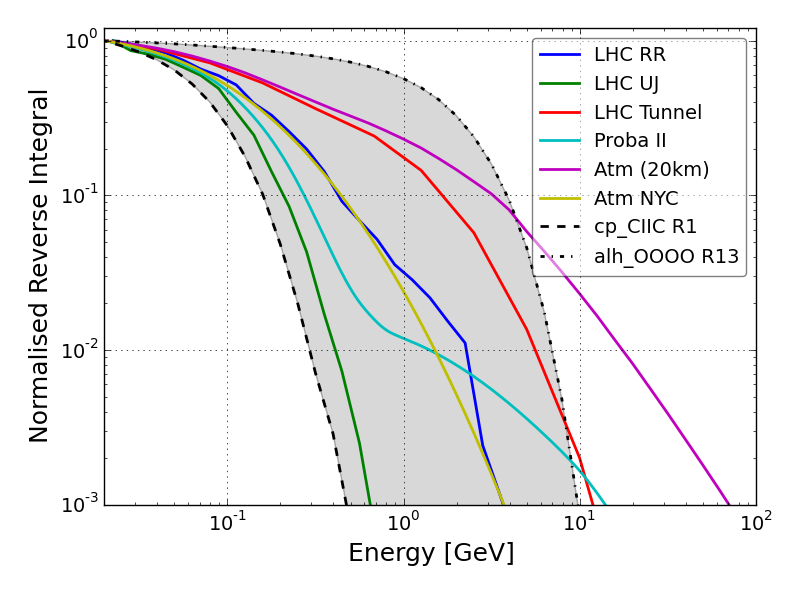
\includegraphics[width=0.7\textwidth]{./images/hardness/all_env_charm}
	\caption{A plot of the reverse integral spectra for test positions at CHARM (in grey), compared with different radiation environments, normalised to 20 MeV.}
	\label{fig:example_rev_spectra}
\end{figure}

\begin{figure}[ht!]
	\centering
	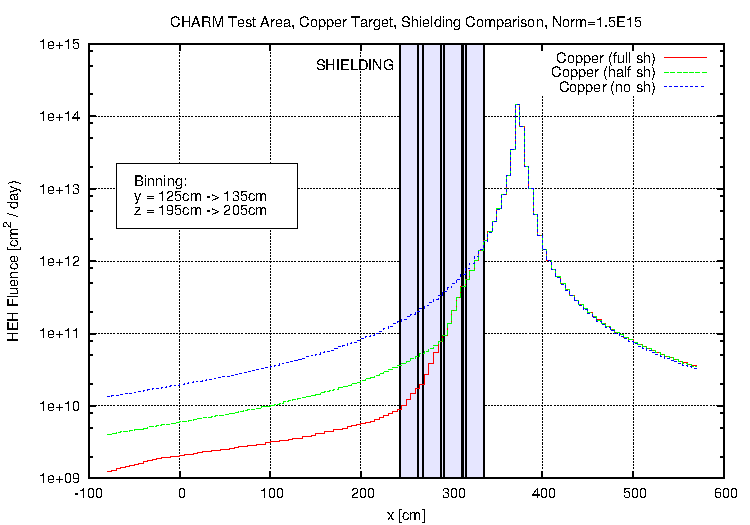
\includegraphics[scale=1.1]{./images/heh_comparison_with_shielding}
	\caption{A plot of the HEH fluence for a slice in the test area geometry from the target, towards the entrance. It shows that with the shielding, there is a reduction in the HEH fluence of a factor 10.}
	\label{fig:HEH_copper_shielding}
\end{figure}

\begin{figure}[ht!]
	\centering
	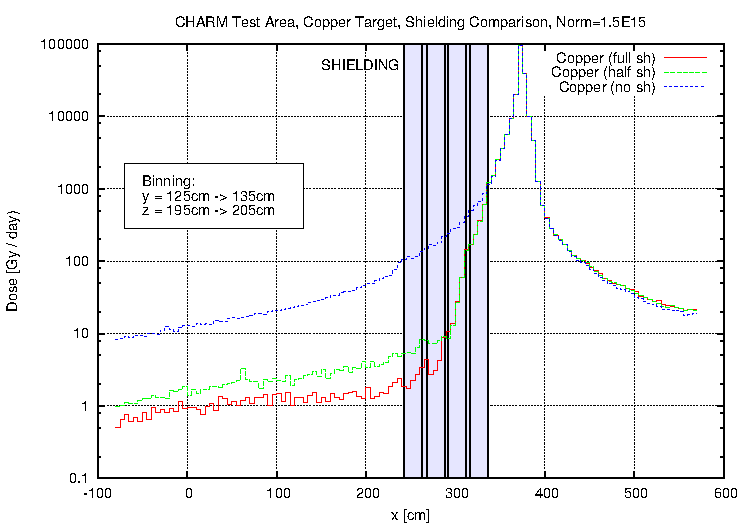
\includegraphics[scale=1.1]{./images/dose_comparison_with_shielding}
	\caption{A plot of the dose for a slice in the test area geometry from the target, towards the entrance. The shielding reduces the dose by almost a factor 100 close to the shielding, and reduces down to a factor 10 by the test positions.}
	\label{fig:dose_copper_shielding}
\end{figure}

\clearpage

\begin{figure}[ht!]
	\centering
	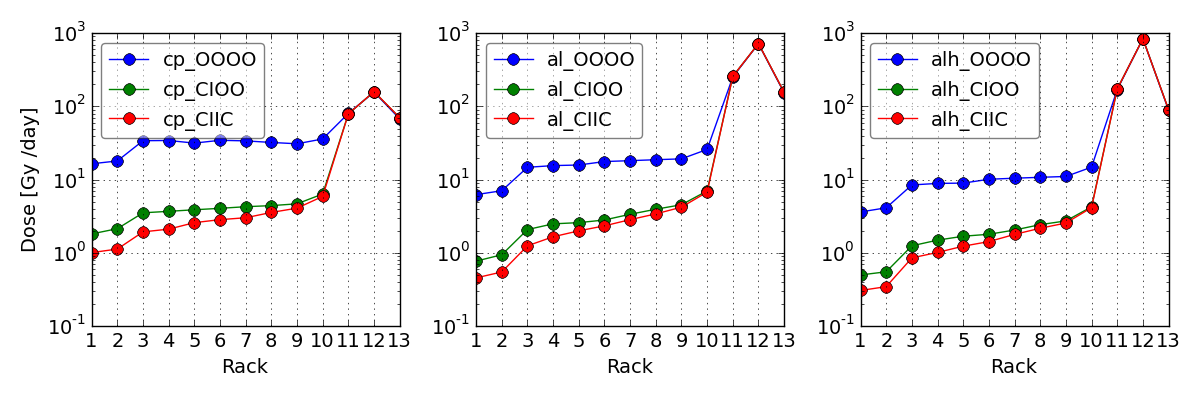
\includegraphics[width=\textwidth]{./images/test_positions/dose_per_day}
	\caption{A plot of the dose per day at the different test positions with the different facility configurations.}
	\label{fig:dose_test_pos}
\end{figure}

\begin{figure}[ht!]
	\centering
	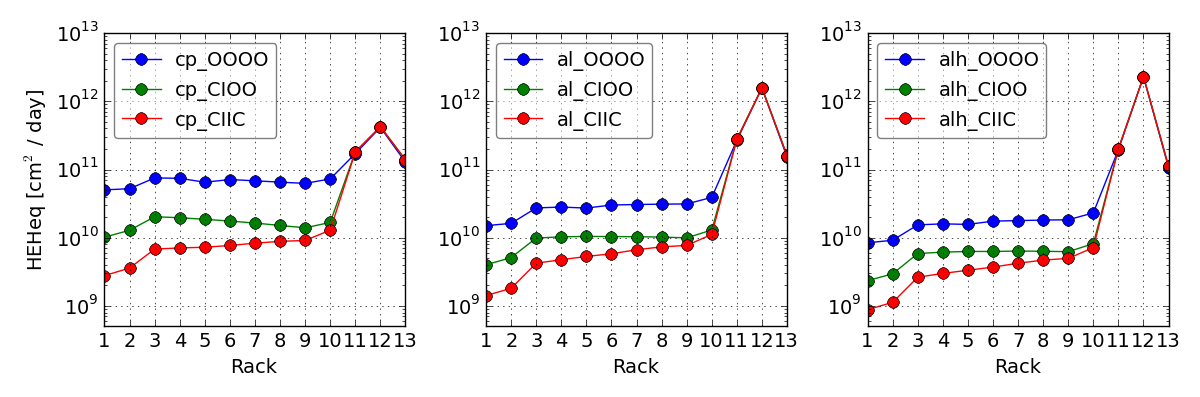
\includegraphics[width=\textwidth]{./images/test_positions/heheq_per_day}
	\caption{A plot of the high energy hadron fluence per day at the different test positions with the different facility configurations.}
	\label{fig:dose_test_pos}
\end{figure}

\clearpage

\subsection{Hardness Factors}

The hardness factors for each test position and configuration have been calculated using the reverse integral of the HEH fluence (see previous chapter for more details on the hardness factors). The same values have also been calculated from data-sets measured (and in some cases simulated) of real environments ranging from accelerator alcove areas where control electronics may be placed, to upper atmospheric and space environments where for example electronics on satellites are exposed to mixed-field radiation environments much harsher than those found at ground level. These two sources of information have been compared in order to find the places at CHARM to test electronics in the same environments they would be used in. This would then give the best indication of their sensitivity (or tolerance) to radiation by exposing them to radiation fields as similar as possible to their intended application. \\

The method to choose the best match is based on trying to find the test positions at CHARM that have the same hardness factors as the desired mixed-field. This is achieved by finding the hardness factors for the desired field, and calculating the difference for each possible test position and configuration at CHARM. The resulting data-table is then sorted to minimise the difference between the value for each hardness factor. Depending on the application, the best match can change. An example of this is when trying to find a test position which is exposed to particle energies of the same magnitude as the desired mixed-field, where there may be a compromise between matching the high energy of the field, and getting correct proportion of lower energy particles. This will depend on the test device and it's error rate as a function of energy. \\

For radiation environments around the HEH LHC, as number of matches have been found. A plot of the reverse integral spectra for a number of simulated LHC environments are shown in figure \ref{fig:lhc_charm_comparison}. These radiation fields could be considered as typical accelerator mixed-field environments, where the UJ and RR areas correspond to shielded areas near the beam-line, and the tunnel area as an un-shielded environment exposed to high energy particle showers from direct beam losses on the beam-line elements. \\

% Reference for data, elias simulations. Table of hardness factors and CHARM matches. Use the ipython notebook to get the hardness factors for the specific cases. Hopefully they match the table in the previous chapter. If not, which should we use??

\begin{table}[htbp]
\centering
\begin{tabular}{l|c|l|l|l}
\textbf{Environment} & \textbf{HEH /cm$^{2}$/ y} & \multicolumn{3}{c}{\textbf{Hardness Factor}} \\ \cline{3-5}
				& & H50   & H10   & H1 \\
\hline
\hline
Proba II (800km, 98$^{o}$)		& 2.7E+09 & 0.094 & 0.273 & 1.406 \\
Atm (20km)						& 3.8E+07 & 0.20  & 3.242 & 17.814 \\
Ground (NYC)					& 1.0E+05 & 0.103 & 0.442 & 1.506 \\
LHC UJ							& 2.5E+09 & 0.087 & 0.212 & 0.421 \\
LHC RR							& 1.0E+09 & 0.116 & 0.431 & 2.312 \\
LHC Tunnel						& 6.0E+11 & 0.19  & 1.901 & 6.56 \\
\end{tabular}%
\caption{A table of hardness factors for the reference spectra used for comparisons with the CHARM test positions. The hardness factors are in units of GeV.}
\label{tab:hardness_factor_references}%
\end{table}%

\newpage

\begin{figure}[ht!]
	\centering
	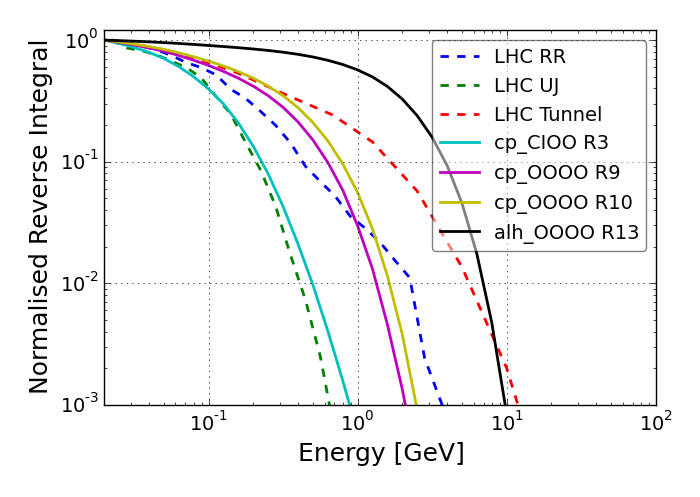
\includegraphics[width=0.7\textwidth]{./images/hardness/lhc_charm_comparison}
	\caption{A plot of several reverse integral spectra from simulations of LHC environments, along with matching CHARM test configurations.}
	\label{fig:lhc_charm_comparison}
\end{figure}

\begin{table}[htbp]
\centering
\begin{tabular}{l|l|l|l}
\textbf{environment} & \multicolumn{3}{c}{\textbf{Hardness Factor}} \\ \cline{2-4}
				& H50   & H10   & H1 \\
\hline
\hline
\rowcolor{gray!30} LHC UJ & 0.087 & 0.212 & 0.421 \\
cp\_CIOO R3	& 0.079 & 0.232 & 0.498 \\

\hline
\rowcolor{gray!30} LHC RR & 0.116 & 0.431 & 2.312 \\
cp\_OOOO R9  & 0.152 & 0.628 & 1.378 \\
cp\_OOOO R10 & 0.190 & 0.782 & 1.665 \\

\hline
\rowcolor{gray!30} LHC Tunnel & 0.19  & 1.901 & 6.56 \\
alh\_OOOO R13 & 1.249 & 3.898 & 7.273 \\
\end{tabular}%
\caption{}
\label{tab:hardness_factor_lhc}%
\end{table}%

\clearpage

\begin{figure}[ht!]
	\centering
	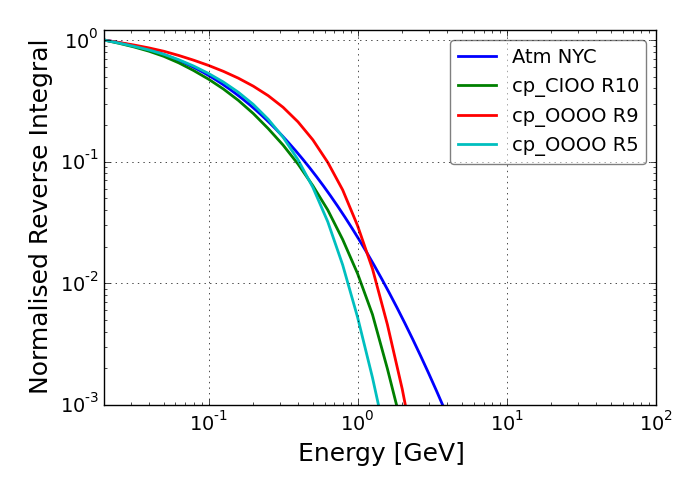
\includegraphics[width=0.7\textwidth]{./images/hardness/atm0km_charm_comparison}
	\caption{A plot of the reverse integral HEH spectrum at ground level (New York, Jedec89 Standard), with a number of CHARM test configurations with close matches.}
	\label{fig:atm0km_charm_comparison}
\end{figure}

\begin{table}[htbp]
\centering
\begin{tabular}{l|l|l|l}
\textbf{environment} & \multicolumn{3}{c}{\textbf{Hardness Factor}} \\ \cline{2-4}
				& H50   & H10   & H1 \\
\hline
\hline
\rowcolor{gray!30} Ground (NYC) & 0.103 & 0.442 & 1.506 \\
cp\_CIOO R10	& 0.094 & 0.389 & 1.080 \\
cp\_OOOO R9		& 0.152 & 0.628 & 1.378 \\
cp\_OOOO R5 	& 0.110 & 0.407 & 0.890 \\
\end{tabular}%
\caption{}
\label{tab:hardness_factor_atm_nyc}%
\end{table}%

\clearpage

\begin{figure}[ht!]
	\centering
	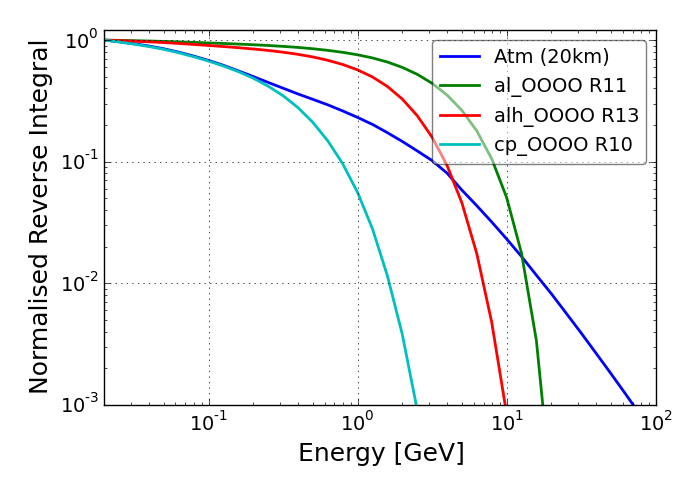
\includegraphics[width=0.7\textwidth]{./images/hardness/atm20km_charm_comparison}
	\caption{A plot of the reverse integral HEH spectrum at an altitude of 20km (Geneva, Switzerland), with a number of CHARM test configurations with close matches. The atmospheric HEH spectra extends to energies beyond those achievable at CHARM, however the intermittent hardness energies can be matched.}
	\label{fig:atm20km_charm_comparison}
\end{figure}

\begin{table}[htbp]
\centering
\begin{tabular}{l|l|l|l}
\textbf{environment} & \multicolumn{3}{c}{\textbf{Hardness Factor}} \\ \cline{2-4}
				& H50   & H10   & H1 \\
\hline
\hline
\rowcolor{gray!30} Atm (20km) & 0.200 & 3.242 & 17.814 \\
al\_OOOO R11	& 2.695 & 8.153 & 14.337 \\
alh\_OOOO R13	& 1.249 & 3.898 & 7.273 \\
cp\_OOOO R10 	& 0.190 & 0.782 & 1.665 \\
\end{tabular}%
\caption{}
\label{tab:hardness_factor_atm_nyc}%
\end{table}%

\clearpage

\begin{figure}[ht!]
	\centering
	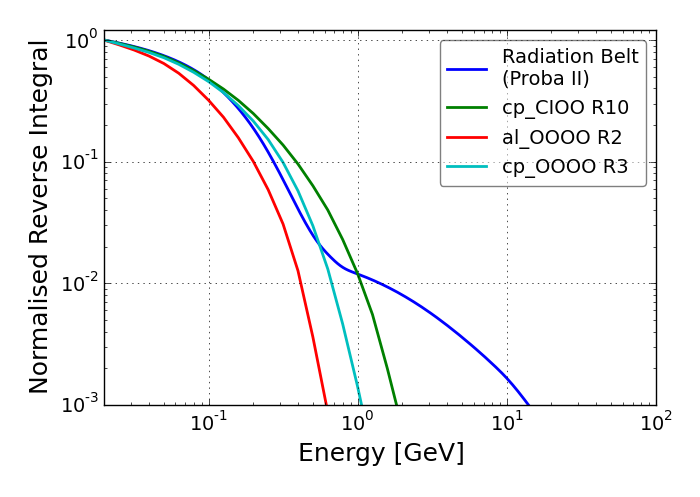
\includegraphics[width=0.7\textwidth]{./images/hardness/space_charm_comparison}
	\caption{A plot of the reverse integral HEH spectrum for the proton belt (Proba II orbit), with a number of CHARM test configurations with close matches.}
	\label{fig:space_charm_comparison}
\end{figure}

\begin{table}[htbp]
\centering
\begin{tabular}{l|l|l|l}
\textbf{environment} & \multicolumn{3}{c}{\textbf{Hardness Factor}} \\ \cline{2-4}
				& H50   & H10   & H1 \\
\hline
\hline
\rowcolor{gray!30} Proba II & 0.094 & 0.273 & 1.406 \\
cp\_CIOO R10	& 0.094 & 0.389 & 1.080 \\
al\_OOOO R2		& 0.068 & 0.200 & 0.428 \\
cp\_OOOO R3 	& 0.090 & 0.314 & 0.691 \\
\end{tabular}%
\caption{}
\label{tab:hardness_factor_proba}%
\end{table}%

\clearpage

\subsection{Copper Target without Shielding}

The following results chapter focuses on the analysis of the calculations using the copper target configuration without shielding (\textbf{cp\_OOOO}). The same tables and plots for the other facility configurations can be found in the appendix. All results tables can also be found at \url{http://thornton.web.HEH.ch/}  \\

The data for all test positions in the cp\_OOOO configuration are shown in table \ref{tab:cpOOOO-alldata}. The results include dose and HEH fluence rates per day (normalised for 1.5E15 protons), spectra content as a percentage of the total HEH fluence, 'R' factors and hardness factors. \\

An example plot of the spectra seen at a test location is shown in figure \ref{fig:cpOOOO_spectra}. the plot shows the relative fluences (arbitrary values) for a range of different particles. Of particular interest is the neutron spectrum which typically has a much larger energy range than the other particles, and is strongly influenced by the shielding and position of the test device. \\

The dose and HEH fluence varies largely depending on the position within the test area, and this is shown in figures \ref{fig:cpOOOO_dosemap} and \ref{fig:cpOOOO_HEHmap}. The plots show the dose and HEH fluence mapped out at the beam height for the whole test area. Large gradients can be seen at the test positions close to the beam axis, therefore testing in these positions should be analysed and set-up carefully, ideally with small test equipment to minimise the variation within the device. Some 'shadows' can be seen in the HEH fluence due to the interaction with the shielding support beams. This is true for all targets, but has less of an impact when using the shielding. \\

\begin{table}[htbp]
\centering
\begin{tabular}{c|P{1.7cm}|P{1.7cm}|c|c|c|c|c|c|c|c}
\textbf{Rack} & \textbf{Dose Gy/ day} & \textbf{HEH /cm$^{2}$/ day} & \multicolumn{4}{c|}{\textbf{Composition}} & \textbf{R} & 				\multicolumn{3}{c}{\textbf{Hardness energy}} \\ \cline{4-7} \cline{9-11}  
& & & n & p & $\pi^{\pm}$ & k & & H50 & H10 & H1 \\
\hline
\hline
1	&	1.65E+01	&	5.03E+10	&	82.90	&	7.04	&	9.54	&	0.20	&	3.48	&	0.06	&	0.18	&	0.38	\\
2	&	1.81E+01	&	5.23E+10	&	82.50	&	7.08	&	9.80	&	0.23	&	3.15	&	0.06	&	0.19	&	0.41	\\
3	&	3.41E+01	&	7.53E+10	&	72.40	&	13.00	&	14.00	&	0.44	&	2.05	&	0.09	&	0.31	&	0.69	\\
4	&	3.43E+01	&	7.44E+10	&	70.30	&	13.70	&	15.30	&	0.49	&	2.06	&	0.10	&	0.36	&	0.78	\\
5	&	3.16E+01	&	6.52E+10	&	69.80	&	13.80	&	15.70	&	0.57	&	2.37	&	0.11	&	0.41	&	0.89	\\
6	&	3.46E+01	&	7.13E+10	&	66.40	&	15.60	&	17.10	&	0.62	&	2.19	&	0.12	&	0.47	&	0.99	\\
7	&	3.39E+01	&	6.84E+10	&	64.90	&	16.10	&	18.10	&	0.70	&	2.30	&	0.13	&	0.51	&	1.12	\\
8	&	3.23E+01	&	6.53E+10	&	63.20	&	16.70	&	19.20	&	0.74	&	2.39	&	0.14	&	0.58	&	1.23	\\
9	&	3.10E+01	&	6.26E+10	&	62.30	&	16.80	&	19.90	&	0.83	&	2.51	&	0.15	&	0.63	&	1.38	\\
10	&	3.61E+01	&	7.28E+10	&	58.80	&	17.20	&	22.70	&	1.11	&	2.05	&	0.19	&	0.78	&	1.67	\\
11	&	8.04E+01	&	1.71E+11	&	34.50	&	23.50	&	37.70	&	4.06	&	0.74	&	1.79	&	6.84	&	12.60	\\
12	&	1.57E+02	&	4.15E+11	&	24.50	&	49.10	&	23.60	&	2.60	&	0.30	&	7.01	&	23.00	&	24.00	\\
13	&	6.77E+01	&	1.28E+11	&	41.30	&	19.50	&	35.60	&	3.41	&	1.03	&	0.73	&	3.35	&	6.51	\\
\end{tabular}
\caption{A table of the spectra content and hardness factors for the test area configuration with copper target and without shielding.}
\label{tab:cpOOOO-alldata}%
\end{table}%


\begin{figure}[!ht]
	\centering
	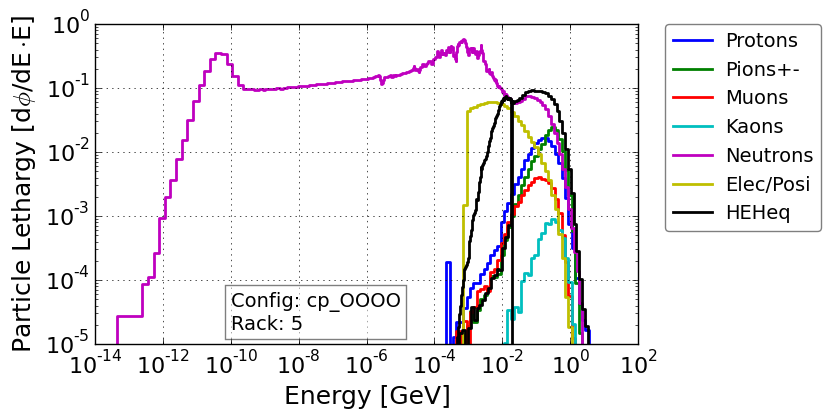
\includegraphics[scale=0.6]{./images/spectra_cp_OOOO_r5}
	\caption{An example plot of the radiation spectra at a test position for the facility configuration with the the copper target without shielding.}
	\label{fig:cpOOOO_spectra}
\end{figure}

\begin{figure}[!ht]
	\centering
	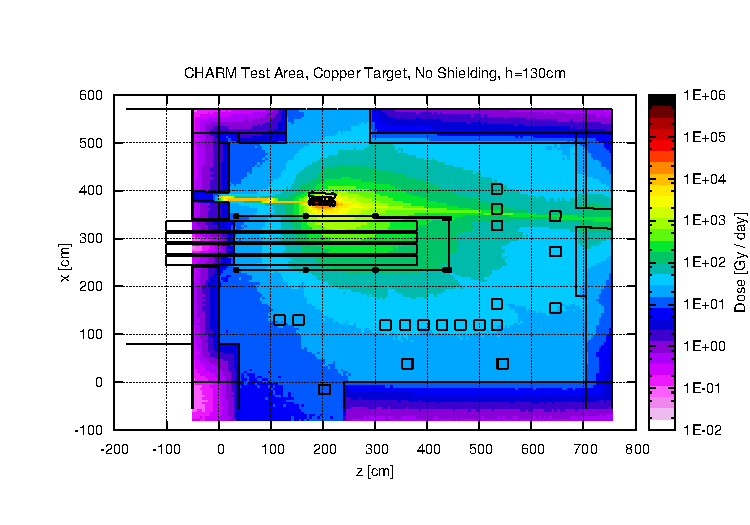
\includegraphics[width=\textwidth]{./images/dose_test_area_cpOOOO}
	\caption{A plot of the dose normalised per day inside the test area at beam height (1.5E15 protons per day).}
	\label{fig:cpOOOO_dosemap}
\end{figure}

\begin{figure}[!ht]
	\centering
	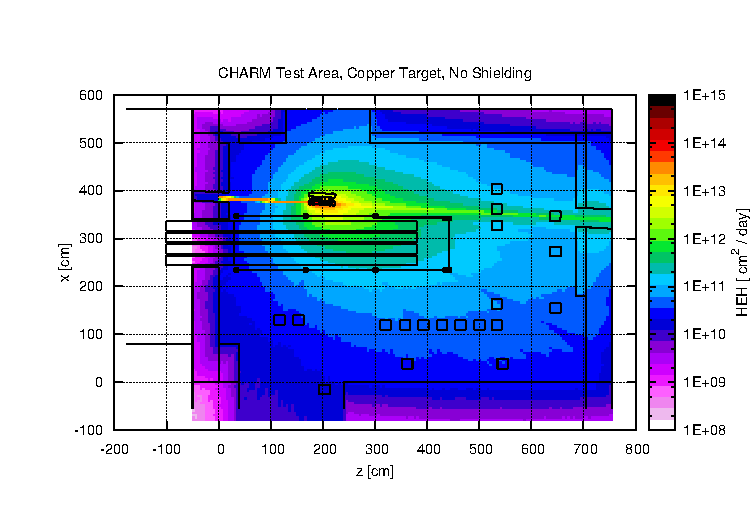
\includegraphics[width=\textwidth]{./images/heh_test_area_cpOOOO}
	\caption{A plot of the HEH fluence normalised per day inside the test area at beam height (1.5E15 protons per day).}
	\label{fig:cpOOOO_HEHmap}
\end{figure}

\clearpage
\subsection{Uncertainties}

There are a number of errors and uncertainties associated with the FLUKA calculations. The first main contributing factor is the accuracy of the geometry. This is in term of position of objects inside the main simulation geometry, materials and dimensions. Secondly there may be errors when comparing the calculations to tests made in the real facility due to positioning, and accurately the device was placed. There needs to be considerations for the test device itself, as the size of the sensitive volume may be large. These points are explored below with the aim of summarizing the various potential errors. \\

The geometry for the CHARM FLUKA calculations was built using the Flair tool \cite{FLAIR1}. Initially it was based on the technical drawings produced for the construction of the facility, however once built it was possible to re-check the dimensions and verify that the drawings were correct. There were some small differences between the drawings and actual construction (for example the back wall build 1m further from the target than initially planned), however these were corrected for the final FLUKA geometry. The bodies in the geometry can be generally considered to be accurate within 1-2cm, with smaller objects such as the target, accurate within 1cm. \\

The accuracy of the test positions within the test facility was also verified during tests of the conveyor system, and can be considered accurate within 1-2cm in each axis. Another error to consider at the test positions is related to the gradients of the radiation, i.e. in positions close to the beam axis, the radiation field can very up to 1\% per centimetre. Therefore the physical size of the test equipment needs to be considered when choosing the test position with the facility. \\

A more detailed analysis of the errors and gradients in the test positions will follow. \\